\documentclass[11pt]{article}
\newcommand{\ReportDate}{30 September 2026}
% Preamble for the roughness technical report. Numbers are NOT typed here:
% they come from ../build/numbers.tex, generated by src/build_report.py.
\usepackage[T1]{fontenc}
\usepackage[utf8]{inputenc}
\usepackage{lmodern}
\usepackage[scaled=0.92]{helvet}
\usepackage[letterpaper,margin=1in,headheight=14pt]{geometry}
\usepackage{microtype}
\usepackage{amsmath}
\usepackage{graphicx}
\usepackage{booktabs,tabularx,array,makecell,longtable,threeparttable}
\usepackage[per-mode=symbol,detect-all]{siunitx}
\usepackage[table]{xcolor}
\usepackage[font=small,labelfont=bf,labelsep=period,justification=raggedright,singlelinecheck=false]{caption}
\usepackage{subcaption}
\usepackage{enumitem}
\usepackage{float}
\usepackage{fancyhdr}
\usepackage{titlesec}
\usepackage{textcomp}
\usepackage{tikz}
\usetikzlibrary{positioning,arrows.meta}
\usepackage[hidelinks]{hyperref}
\hypersetup{pdftitle={Printed surface texture and the electrical output of a small VAWT rotor},
  pdfauthor={Stephen Eacuello}}
\widowpenalty=10000 \clubpenalty=10000
\hyphenation{time-stamps}

\definecolor{ink}{HTML}{0B0B0B}
\definecolor{ink2}{HTML}{52514E}
\definecolor{rule}{HTML}{C9C8C2}
\definecolor{navy}{HTML}{002147}
\definecolor{note}{HTML}{F4F3EF}
\definecolor{gold}{HTML}{B8860B}

\sisetup{group-minimum-digits=5, round-mode=none}
\setlist{nosep, leftmargin=1.4em}
\setlength{\parskip}{0.45em}
\setlength{\parindent}{0pt}
\renewcommand{\arraystretch}{1.12}

\titleformat{\section}{\normalfont\sffamily\Large\bfseries\color{navy}}{\thesection}{0.6em}{}
\titleformat{\subsection}{\normalfont\sffamily\large\bfseries\color{navy}}{\thesubsection}{0.6em}{}
\titleformat{\subsubsection}{\normalfont\sffamily\normalsize\bfseries}{\thesubsubsection}{0.6em}{}
\titlespacing*{\section}{0pt}{1.2em}{0.5em}
\titlespacing*{\subsection}{0pt}{1.0em}{0.35em}

\pagestyle{fancy}
\fancyhf{}
\fancyhead[L]{\sffamily\footnotesize\color{ink2}Printed surface texture and VAWT electrical output}
\fancyhead[R]{\sffamily\footnotesize\color{ink2}\ReportDate}
\fancyfoot[C]{\sffamily\footnotesize\color{ink2}\thepage}
\renewcommand{\headrulewidth}{0.4pt}

% A shaded box for the bottom line.
\newsavebox{\keyboxbin}
\newenvironment{keybox}{\par\smallskip\noindent\begin{lrbox}{\keyboxbin}%
  \begin{minipage}{\dimexpr\linewidth-2\fboxsep-1.2pt\relax}}%
  {\end{minipage}\end{lrbox}\fcolorbox{rule}{note}{\usebox{\keyboxbin}}\par\smallskip}

\newcommand{\Ra}[1]{\ensuremath{\mathrm{Ra}\,#1}}
\newcommand{\pmax}{P_{\max}}
\newcommand{\figref}[1]{Fig.~\ref{#1}}
\newcommand{\tabref}[1]{Table~\ref{#1}}
\newcommand{\secref}[1]{Section~\ref{#1}}
\newcommand{\appref}[1]{Appendix~\ref{#1}}
% \input is not expandable, which breaks it between booktabs rules; @@input is.
\makeatletter\newcommand{\tabinput}[1]{\@@input #1 }\makeatother

\input{../build/numbers}
\newcommand{\TODO}[1]{\textcolor{red}{\textbf{[TODO: #1]}}}
\graphicspath{{../build/fig/}}

\begin{document}

% ------------------------------------------------------------------ title --
\thispagestyle{empty}
\begin{flushleft}
{\sffamily\small\color{ink2} TECHNICAL REPORT \quad·\quad UNIVERSITY OF RHODE ISLAND}\\[0.8em]
{\sffamily\LARGE\bfseries\color{navy} Printed surface texture and the electrical output\\[0.15em] of a small vertical-axis wind turbine rotor}\\[0.5em]
{\sffamily\large Wind-tunnel results, August–September 2026}\\[1.0em]
{\small
\begin{tabular}{@{}ll@{}}
\textbf{Prepared by} & Stephen Eacuello \\
\textbf{For}         & Prof.\ Vahid Jahangiri, Prof.\ Yeonho Jeong, Prof.\ Manbir Sodhi, Taegu Kang \\
\textbf{Date}        & \ReportDate \\
\textbf{Data}        & \texttt{URI\_VAWT\_Roughness\_Data\_2026-09-30.zip} (accompanies this report)
\end{tabular}}
\end{flushleft}
\vspace{0.2em}
{\color{rule}\hrule height 0.6pt}

% ---------------------------------------------------------------- summary --
\section*{Summary}

\begin{keybox}
\textbf{Bottom line.} On one mounting each, rotors printed with \SI{0.10}{} and
\SI{0.20}{mm} of fuzzy-skin texture produced about 8\% and 14\% more peak electrical power
than the \SI{0.05}{mm} rotor across \vlo–\vhi{}\,\si{m/s}. The extra power comes with the
rotor turning faster in the same wind, not from the electrical side. It is not yet shown that
texture, rather than mounting, print differences or a change between the first run and the
others, is the cause. \ifHaveRepeat The 1~October remounts (\secref{sec:repeat}) are the first check. \else The remounts planned for 1~October are the first check.\fi
\end{keybox}

\begin{table}[h]
\centering\small
\begin{tabular}{@{}l c c c c@{}}
\toprule
Rotor (label) & Fuzzy-skin thickness & $\pmax$ at \vhi{}\,m/s & Change vs \Ra{20} & 95\% CI$^\ast$ \\
\midrule
\Ra{20} & \SI{0.050}{mm} & \SI{\pmaxtopA}{W} & — & — \\
\Ra{40} & \SI{0.101}{mm} & \SI{\pmaxtopB}{W} & $\lvlABraw\%$ & $[\lvlABrawloar,\ \lvlABrawhiar]$ \\
\Ra{80} & \SI{0.202}{mm} & \SI{\pmaxtopC}{W} & $\lvlACraw\%$ & $[\lvlACrawloar,\ \lvlACrawhiar]$ \\
\bottomrule
\end{tabular}\\[2pt]
{\footnotesize $^\ast$Change is the geometric mean over 14 wind speeds. The interval covers
scatter between wind speeds within a single mounting, allowing for correlation between
neighbouring points. It does not cover mount-to-mount variation.}
\end{table}

\begin{itemize}[leftmargin=1.2em]
  \item \textbf{Consistency.} \Ra{80} is higher than \Ra{20} at all 14 wind speeds, and \Ra{40}
        at 13, the fourteenth being equal to within \SI{\tiemw}{mW} (\figref{fig:ratio}). \Ra{80} is higher than
        \Ra{40} by $\lvlBCraw\%$ ($[\lvlBCrawloar,\ \lvlBCrawhiar]$). \Ra{40} and \Ra{80}
        were both tested after a round of software and firmware changes, so that comparison is
        free of the one confound that sets \Ra{20} apart (\secref{sec:discussion}).
  \item \textbf{Mechanism.} The textured rotors' open-circuit voltage, which tracks
        free-running rotor speed, is higher at every wind speed ($\vocB\%$ and $\vocC\%$),
        while the apparent source resistance is unchanged (\secref{sec:thevenin}). For
        \Ra{80} the advantage grows with wind speed, from about $\voclowC\%$ below
        \SI{17}{m/s} to $\vochighC\%$ above \SI{31}{m/s}.
  \item \textbf{Caveats.}
        \ifHaveRepeat Remounting \remountlist{} gives the mount-to-mount variation;
        including it, the changes relative to \Ra{20} are \macmplist. \else Each rotor was
        mounted once. \fi
        The Ra labels are targets estimated when the prints were planned, never measured
        (\secref{sec:specimens}). The rig measures electrical power, not the aerodynamic
        power coefficient, and it did not record rotor speed.
\end{itemize}

\textbf{Responses to open requests.}
\begin{itemize}[leftmargin=1.2em]
  \item \emph{Comparison with the initial test (Prof.\ Jeong, 27 July).} Over 800–1700 rpm the
        5 June values lie between $\junAlo\%$ and $\junAhi\%$ of the rig's \Ra{20}
        (geometric mean $\junAmid\%$), within the range the three textured rotors span
        (\secref{sec:jeong}). The rotor and the processing differ, so this is a consistency
        check, not a texture comparison.
  \item \emph{The 27 July no-texture test.} Reprocessed from its raw export, it cannot resolve a
        difference of 8–14\% (\secref{sec:jeong}). \ifHaveSmooth The no-texture rotor has now
        also been run on the rig. \else Running the same rotor on the rig is the direct
        comparison. \fi
  \item \emph{Which blade exactly (Prof.\ Jahangiri, 27 July).} \secref{sec:specimens} lists
        what is known about each rotor, including what is still inferred.
  \item \emph{Fault-testing plan (Prof.\ Jeong, 15 and 27 July).} Not yet drafted. A starting
        point is proposed in \secref{sec:faults}.
\end{itemize}

\textbf{Acknowledgement.} Taegu Kang co-ran the 27 July, 20 August and 26 August tests, and
shared the complete raw export of the July test, without which \secref{sec:jeong} would not
have been possible.

{\setlength{\parskip}{0pt}\setcounter{tocdepth}{1}\small\tableofcontents}
\clearpage

% ============================================================== 1 SCOPE ==
\section{Objective and scope}

The question is whether the surface texture of 3D-printed blades changes the power a small
vertical-axis wind turbine (VAWT) can deliver, and by how much. This report covers every
texture test run on the automated rig to date. It places the Jeong-lab tests of June and July
in context, states what the data do and do not support, and lists the measurements that would
close the remaining gaps. The accompanying data package contains every raw file used,
unmodified, together with a data dictionary, checksums and the analysis code
(\appref{app:package}). Every number in this report is generated from those files.

\begin{figure}[t]
  \centering
  \includegraphics[width=\linewidth]{fig_ratio}
  \caption{Change in peak electrical power (raw arg\,max basis) relative to the \Ra{20} rotor
  at each of the 14 matched fan set points. Horizontal lines: geometric-mean change. Shaded bands: 95\%
  intervals that assume independent set points (\secref{sec:stats} gives the wider intervals
  that allow for correlation).}
  \label{fig:ratio}
\end{figure}

% =========================================================== 2 SPECIMENS ==
\section{Test articles}\label{sec:specimens}

\subsection{Rotor}
The rotor is a three-bladed VAWT with straight blades on arms (\tabref{tab:rotor}). Its
blade section is not an airfoil. Each blade is a thin cambered plate: a constant
\SI{1.79}{mm} wall, about \SI{24.5}{mm} deep overall on a \SI{48}{mm} chord, \SI{183}{\degree}
of turning and square-cut edges, prismatic along the span with no twist. In cross-section
each blade is closer to a half-cylinder bucket than to a wing. Because a VAWT sweeps a
cylinder, the swept area is $A=2RH$.

\begin{table}[t]
\centering\small
\caption{Rotor geometry (common to all test rotors; from the blade mesh).}\label{tab:rotor}
\begin{tabular}{@{}ll@{}}
\toprule
Configuration & 3 straight blades, zero twist \\
Radius $R$ (axis to blade attachment) & \SI{0.1016}{m} \\
Span $H$ & \SI{0.2451}{m} \\
Swept area $2RH$ & \SI{0.0498}{m^2} \\
Chord $c$ & \SI{48}{mm} \\
Section & cambered plate, \SI{1.79}{mm} wall, square edges, \SI{183}{\degree} turning \\
Chord Reynolds number & $\relo\times10^4$ to $\rehi\times10^5$ (nominal wind, air at \SI{20}{\celsius}) \\
\bottomrule
\end{tabular}
\end{table}

\subsection{The texture specimens, and what is known about each}
All textured rotors are printed copies of geometry \texttt{v1}, the first printed replica of the
original rotor, which the professors chose over a remodelled \texttt{v2} on 4 August. They
differ in the slicer's fuzzy-skin setting, which randomly displaces the outer wall. The
controlled variable is the fuzzy-skin \emph{thickness}, and it doubles from one rotor to the
next (\tabref{tab:specimens}).

\begin{table}[t]
\centering\small
\caption{The rotors in this report. Thicknesses of the textured sets were confirmed by the
operator. The Ra labels are not measurements (see text).}\label{tab:specimens}
\begin{tabularx}{\linewidth}{@{}l l l X@{}}
\toprule
Rotor & Texture & Tested & Known / inferred \\
\midrule
Initial reference & — & 5 Jun (lab) & Probably the rotor used before the printed replicas, which were finished 13 July. Not confirmed. \\
No texture & none & 27 Jul (lab)\ifHaveSmooth, 1 Oct (rig)\fi & Printed replica without fuzzy skin (``the new blades which have no texture''). Geometry probably \texttt{v1}; to be confirmed by T.~Kang. \\
\ifHaveRaTen \Ra{10} & \SI{0.025}{mm}\ifRaTenConfirmed\else$^\ast$\fi & 1 Oct (rig) & \ifRaTenConfirmed Confirmed. \else$^\ast$Identity not yet confirmed; shown but excluded from every trend fit. \fi \\ \fi
\Ra{20} & \SI{0.050}{mm} & 20 Aug (rig) & Printed in the garage on a Bambu printer with a \SI{0.4}{mm} nozzle and \SI{0.08}{mm} layers. The run was first logged as \texttt{v2\_Ra20} and relabelled; the data are unchanged. \\
\Ra{40} & \SI{0.101}{mm} & 1 Sep (rig) & Same garage print batch as \Ra{20}. Carried a small magnet on one blade for a reed-switch rotor-speed sensor. \\
\Ra{80} & \SI{0.202}{mm} & 26 Aug (rig) & Printer, nozzle and layer not recorded. \\
\bottomrule
\end{tabularx}
\end{table}

Four facts about the specimens limit how the results can be read.
\begin{itemize}
  \item \textbf{The Ra values are labels, not measurements.} ``\Ra{20}'' and ``\Ra{40}'' are
        the roughness targets that an AI assistant (ChatGPT) suggested on 4 August for
        thicknesses of 0.050 and \SI{0.101}{mm}. That same table put \SI{0.025}{mm} at
        \Ra{10}. ``\Ra{80}'' was never in that table: it extends the doubling. A second AI
        estimate (12 August) put the 0.050 and \SI{0.101}{mm} settings at about 10–15 and
        20–35\,\si{\micro m}, one-half to three-quarters of the labels. No surface has been measured. This report uses fuzzy-skin
        thickness as the texture variable.
  \item \textbf{The print details typed into the run notes are not reliable.} The notes say
        ``0.2mm layer'' and, for \Ra{80}, ``0.2mm nozzle''. The garage printer had only
        \SI{0.4}{mm} nozzles throughout the campaign, and the person who printed the sets
        reported \SI{0.08}{mm} layers. The slicer project files are archived but have not yet
        been read.
  \item \textbf{The prints came from more than one source.} Nothing records which print file
        produced which rotor, and on 13 August two print sets were noted to ``feel very
        different''. If the rotors differ in mass, wall thickness or edge finish as well as
        in texture, those differences are confounded with texture here.
  \item \textbf{The \Ra{40} rotor carried a small magnet} on one blade for the reed switch; the
        others, as far as the records show, did not.
\end{itemize}

% ============================================================= 3 METHOD ==
\section{Facility, instrumentation and protocol}\label{sec:method}

\subsection{Rig}
\figref{fig:rig} shows the chain used for the rotor sweeps. A Python host commands the tunnel
fan through a Portenta Machine Control and an ABB ACS550 drive. The generator on the rotor
shaft feeds a three-phase bridge rectifier. A Chroma 63004 DC electronic load, controlled
by the same host, sets the load current and measures terminal voltage and current. Wind speed
comes from the tunnel calibration $v = 0.02132\,N_\text{fan} - 0.424$ (\si{m/s}, fan speed
$N_\text{fan}$ in rpm, $R^2=0.9996$), applied to the \emph{commanded} fan speed
(\secref{sec:quality}).

\begin{figure}[t]
  \centering
  % Measurement and control chain used for the rotor sweeps (drawn for this report).
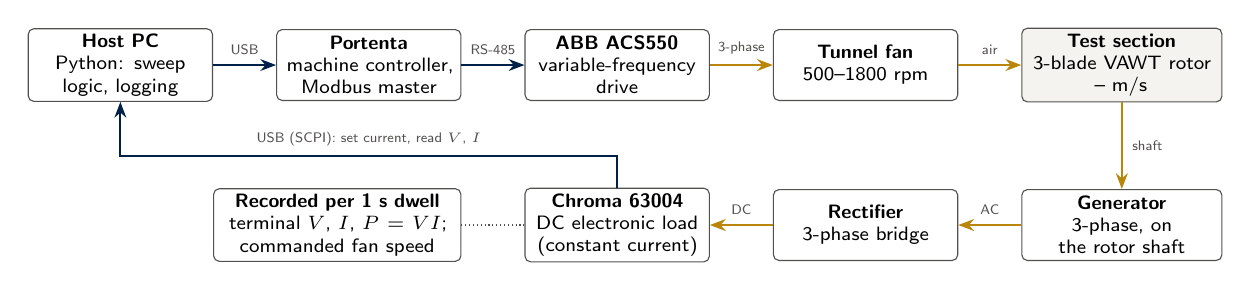
\begin{tikzpicture}[
    font=\sffamily\scriptsize,
    box/.style={draw=ink2, rounded corners=2pt, fill=white, minimum height=9mm,
                text width=22mm, align=center, inner sep=2pt,
                execute at begin node={\hyphenpenalty=10000\exhyphenpenalty=10000}},
    ctl/.style={-{Stealth[length=2mm]}, draw=navy, line width=0.7pt},
    pwr/.style={-{Stealth[length=2mm]}, draw=gold, line width=0.9pt},
    lab/.style={font=\sffamily\tiny, text=ink2},
    node distance=5mm and 8mm]
  % control row
  \node[box] (host) {\textbf{Host PC}\\Python: sweep logic, logging};
  \node[box, right=of host] (pmc) {\textbf{Portenta}\\machine controller, Modbus master};
  \node[box, right=of pmc] (vfd) {\textbf{ABB ACS550}\\variable-frequency drive};
  \node[box, right=of vfd] (fan) {\textbf{Tunnel fan}\\500--1800 rpm};
  \node[box, right=of fan, fill=note, text width=24mm] (ts) {\textbf{Test section}\\3-blade VAWT rotor\\\vlo--\vhi{} m/s};
  % measurement row
  \node[box, below=11mm of ts, text width=24mm] (gen) {\textbf{Generator}\\3-phase, on the rotor shaft};
  \node[box, left=of gen] (rect) {\textbf{Rectifier}\\3-phase bridge};
  \node[box, left=of rect] (load) {\textbf{Chroma 63004}\\DC electronic load (constant current)};
  \node[box, left=of load, text width=30mm] (note) {\textbf{Recorded per 1 s dwell}\\terminal $V$, $I$, $P=VI$;\\commanded fan speed};
  % arrows
  \draw[ctl] (host) -- node[above, lab] {USB} (pmc);
  \draw[ctl] (pmc) -- node[above, lab] {RS-485} (vfd);
  \draw[pwr] (vfd) -- node[above, lab] {3-phase} (fan);
  \draw[pwr] (fan) -- node[above, lab] {air} (ts);
  \draw[pwr] (ts) -- node[right, lab] {shaft} (gen);
  \draw[pwr] (gen) -- node[above, lab] {AC} (rect);
  \draw[pwr] (rect) -- node[above, lab] {DC} (load);
  \draw[ctl] (load.north) |- ++(0,4mm) -| node[pos=0.25, above, lab] {USB (SCPI): set current, read $V$, $I$} (host.south);
  \draw[densely dotted, ink2] (load) -- (note);
\end{tikzpicture}

  \caption{Measurement and control chain used for the rotor sweeps. Rotor speed was not
  recorded.}
  \label{fig:rig}
\end{figure}

\subsection{Sweep protocol}
All rig runs used one automated protocol. The software identifies it by the fingerprint
\texttt{94bed28333f7}, which it computes from every setting that affects what a measurement
means. For each of 14 fan set points from 500 to 1800 rpm in steps of 100:
\begin{enumerate}
  \item the fan is commanded, and the host waits for the drive to reach speed and for the
        terminal voltage to settle;
  \item the load steps its constant-current demand upward, dwelling \SI{1.0}{s} per step and
        recording voltage and current at the end of each dwell. The step is \SI{20}{mA} at
        1800 rpm and scales with $v^2$ at lower wind, so every wind speed gets a comparable
        number of steps;
  \item the ramp stops at the first step where power falls below 80\% of the running maximum
        (the last step in these runs was at \rolloffmin–\rolloffmax\% of the peak), the load
        is released, and the fan steps up.
\end{enumerate}
A run takes about eight minutes.

\subsection{Peak power: two estimators}
Two estimates of $\pmax$ come from each load ladder.
\begin{itemize}
  \item The \emph{raw arg\,max} is the largest single dwell.
  \item The \emph{parabolic fit} is the vertex of a least-squares parabola through the
        arg\,max and the two dwells either side.
\end{itemize}
The top of $P(I)$ is flat, so the arg\,max is biased slightly high. The \Ra{20} run predates
the logged fit, so we recomputed both estimators for every run from its raw dwells, using the
rig's own rule (\appref{app:methods}). The recomputed arg\,max values equal the logged ones
exactly. The recomputed fits match the logged \Ra{40} and \Ra{80} fits to within 0.14\%, which
is the rounding of the stored values. The fit fell back to the arg\,max at \nfallback{} set points (\fallbacklist). The
headline numbers use the raw arg\,max; the two bases agree (\tabref{tab:pairwise}).

\subsection{Statistics}\label{sec:stats}
Rotors are compared at \emph{matched fan set points}. For each pair the change is the geometric
mean of the 14 paired ratios. Two 95\% intervals are given.
\begin{itemize}
  \item The first uses the $t$ distribution on the log-ratios and assumes the 14 set points
        are independent.
  \item They are not. Neighbouring set points share local deviations: the lag-1
        autocorrelation of the log-ratios is \roneACraw{} for \Ra{80} against \Ra{20}. The
        second interval therefore uses an AR(1) effective sample size, and it is the one
        quoted in the Summary.
\end{itemize}
Both intervals describe scatter between wind speeds within one mounting of each rotor. Neither
includes mount-to-mount or print-to-print variation\ifHaveRepeat, which the remounts of
\secref{sec:repeat} address\fi. Counts such as ``higher at 14 of 14'' are likewise not
independent replications: a single offset over a whole run would produce them. The change in
the power-law exponent, $\Delta n$, is the slope of the paired log-ratio against $\ln v$.

% ======================================================= 4 DATA QUALITY ==
\section{Data inventory and quality}\label{sec:quality}

\begin{table}[t]
\centering\small
\caption{All texture-campaign data.}\label{tab:inventory}
\begin{tabularx}{\linewidth}{@{}l l l >{\raggedright\arraybackslash}X@{}}
\toprule
Condition & Date & Source & Status \\
\midrule
\Ra{20} & 20 Aug & rig & \cleanA/14 set points clean, \stepsA{} dwells; predates the fit column and timestamps \\
\Ra{80} & 26 Aug & rig & \cleanC/14 clean, \stepsC{} dwells \\
\Ra{40} & 1 Sep  & rig & \cleanB/14 clean, \stepsB{} dwells; also air temperature and pressure; reed-switch rotor speed not usable \\
\ifHaveRepeat Remounts & 1 Oct & rig & \remountlist \\ \fi
\ifHaveRaTen \Ra{10} & 1 Oct & rig & \cleanT/14 clean \\ \fi
\ifHaveSmooth No texture & 1 Oct & rig & \cleanS/14 clean \\ \fi
No texture & 27 Jul & Jeong-lab DAQ & 360 Hz raw export and summary table (\secref{sec:jeong}) \\
Initial reference & 5 Jun & Jeong-lab DAQ & summary table and plots; raw export not in hand \\
\ifHaveRaTen\else \Ra{10} & — & — & planned, not run (1 Sep tested \Ra{40} instead) \\ \fi
\bottomrule
\end{tabularx}
\end{table}

\textbf{Every set point of every rig run finished cleanly.} The load ramp stopped on the power
roll-off each time, never on the current ceiling or a rotor stall, so every $\pmax$ is a true
maximum rather than a lower bound. All rig runs carry protocol \texttt{94bed28333f7}.

\textbf{Within-mounting repeatability is good.} Two single-point re-measurements of \Ra{20} on
the same mounting (on a different protocol, so indicative only) matched the sweep to within
0.3\% at 1200 and 1800 rpm.

\textbf{Fan-speed logging changed between runs; the fan speed did not.} The \Ra{20} file
records the fan \slipabsA{} rpm below its command, while \Ra{40} and \Ra{80} record it within
\slipabsB{} rpm. For \Ra{20} the software logged the drive's \emph{output frequency} multiplied
by a fixed \SI{29.5}{rpm/Hz}, and all \ragrid{} values fall on that 0.1\,Hz grid. From 25
August it read the drive's own speed estimate. The fan motor current at matched command
agrees across the three runs to within \SI{\motorampsdiff}{A}, which a fan running up to
\SI{21}{rpm} slower would not do. All comparisons are therefore made at matched
\emph{commanded} speed. As a bound only: if the \Ra{20} readback \emph{had} been a real
air-speed deficit, correcting for it would reduce the gains to $\sensB\%$ and $\sensC\%$.

\textbf{Ambient conditions were recorded only for \Ra{40}} (\SI{24.6}{\celsius},
\SI{101.04}{kPa}, sensor offset uncalibrated). On this rig $\pmax$ rises faster than linearly
with dynamic pressure, so a density difference of a few percent between days could shift
$\pmax$ by up to about twice that. This is small next to the \Ra{80} gain but comparable to the
\Ra{80}-vs-\Ra{40} step.

% ============================================================= 5 RESULTS ==
\section{Results}\label{sec:results}

\subsection{Power curves}
\figref{fig:pmax} shows $\pmax$ against wind speed. Peak power rises from about
\SI{0.03}{W} at \vlo{}\,\si{m/s} to \pmaxtopA, \pmaxtopB{} and \pmaxtopC{}\,\si{W} at
\vhi{}\,\si{m/s} for \Ra{20}, \Ra{40} and \Ra{80}. Each curve follows $\pmax \propto v^{n}$
with $n=\nArawexp$, \nBrawexp{} and \nCrawexp{} (\tabref{tab:powerlaw}). \appref{app:data}
tabulates every set point.

\begin{figure}[t]
  \centering
  \includegraphics[width=\linewidth]{fig_pmax}
  \caption{Peak electrical power (raw arg\,max) against nominal wind speed. (a) Linear axes. (b) Log axes
  with a power-law fit per rotor.}
  \label{fig:pmax}
\end{figure}

\subsection{Paired comparison}
\tabref{tab:pairwise} and \figref{fig:ratio} give the paired comparisons. Individual set
points scatter by about 4\%: the standard deviation of the log-ratios is \sdABraw\% for
\Ra{40} and \sdACraw\% for \Ra{80}. A single set point can therefore show anything from
$\minrACraw\%$ to $\maxrACraw\%$ for \Ra{80}.

The largest deviations are at fan 1000–1100 (\SIrange{21}{23}{m/s}). At 1100 rpm both textured
rotors are high ($\exBOneOneZeroZero\%$ and $\exCOneOneZeroZero\%$ against \Ra{20}), which
points to a low \Ra{20} reading there. At 1000 rpm only \Ra{80} is high: it is
$\exCOneZeroZeroZero\%$ over \Ra{20} and $\exBCOneZeroZeroZero\%$ over \Ra{40}, so that point is
specific to \Ra{80}.

\begin{table}[t]
\centering\small
\caption{Paired comparisons at the 14 matched fan set points. CI: 95\% interval assuming
independent set points. CI$_\text{AR}$: allowing for correlation between neighbouring set
points. $\Delta n$: change in the power-law exponent, $\pm$~95\% half-width. Changes in percent.}\label{tab:pairwise}
\footnotesize\setlength{\tabcolsep}{3.5pt}
\begin{tabular}{@{}l l r c c c c c@{}}
\toprule
Comparison & Basis & Change & CI & CI$_\text{AR}$ & Higher & Range & $\Delta n$ \\
\midrule
\tabinput{../build/tables/pairwise_rows.tex}
\bottomrule
\end{tabular}
\end{table}

\subsection{Trend with texture}
Power increases with fuzzy-skin thickness at \monoraw{} of 14 set points
(\figref{fig:trend}). The exception is 700 rpm, where \Ra{40} and \Ra{80} are within
\gapsevenhundred\%. A single slope in log–log coordinates gives
$\pmax\propto t_\text{fuzz}^{\,\betaraw}$, about $\dblraw\%$ per doubling of thickness. No
uncertainty can yet be attached to that slope. It rests on three rotors mounted once each, and
a 3\% offset on the single \Ra{20} mounting would move it by about a quarter.
\ifHaveMountTrend Over all mountings the slope is \mabeta{} (\secref{sec:repeat}). \fi

\begin{figure}[t]
  \centering
  \begin{minipage}[t]{0.49\linewidth}\vspace{0pt}
    \includegraphics[width=\linewidth]{fig_trend}
  \end{minipage}\hfill
  \begin{minipage}[t]{0.47\linewidth}\vspace{6pt}
  \caption{Peak power relative to \Ra{20} against fuzzy-skin thickness. Grey lines:
  individual set points. Markers: geometric mean with 95\% interval (independent set points).
  Black line: the single-slope fit.}
  \label{fig:trend}
  \end{minipage}
\end{figure}

\subsection{Where the extra power comes from}\label{sec:thevenin}
At a fixed wind speed the rotor, generator and rectifier together behave as a Thévenin
source. Across each load ladder the terminal voltage falls linearly with current,
$V = V_\mathrm{oc} - I R_\mathrm{int}$, with $r^2\ge\thevminrtwo$ at every set point of every run.
\begin{itemize}
  \item $V_\mathrm{oc}$ is the zero-current intercept. It tracks the generator EMF, and hence rotor
        speed at light load, to within a rectifier offset of about \SI{0.45}{V}.
  \item $R_\mathrm{int}$ combines the winding, rectifier and wiring with the rotor's slowing under
        load.
  \item At the power maximum $\pmax \approx V_\mathrm{oc}^2/4R_\mathrm{int}$, so a change in power can be
        split between the two.
\end{itemize}

\figref{fig:thevenin} and \tabref{tab:thevenin} show the result.
\begin{itemize}
  \item \textbf{Open-circuit voltage.} The textured rotors' $V_\mathrm{oc}$ is higher at every one
        of the 14 set points: by $\vocB\%$ ($[\vocloB,\ \vochiB]$) for \Ra{40} and $\vocC\%$
        ($[\vocloC,\ \vochiC]$) for \Ra{80}.
  \item \textbf{Source resistance.} Their $R_\mathrm{int}$ is indistinguishable from \Ra{20}'s:
        $\rintB\%$ ($[\rintloB,\ \rinthiB]$) and $\rintC\%$ ($[\rintloC,\ \rinthiC]$).
        Within its uncertainty, the $V_\mathrm{oc}$ change accounts for the whole power gain.
  \item \textbf{A direct check.} The voltage measured at the first, lightest load step, with no
        fitting, is higher by $\vlightB\%$ and $\vlightC\%$, at all 14 set points for both
        rotors.
\end{itemize}

\textbf{At light load the textured rotors turn faster in the same wind, and the extra power
follows from that.} The effect is on the rotor side of the generator, not in the electrical
path. The pattern differs between the two rotors. The \Ra{40} advantage is flat across the
range ($\voclowB\%$ below \SI{17}{m/s}, $\vochighB\%$ above \SI{31}{m/s}). The \Ra{80} advantage
grows with wind speed, from $\voclowC\%$ to $\vochighC\%$: against \Ra{40} its slope in $\ln v$
is $\vocslopeBC$ ($p=\vocslopepBC$). Faster free-running does not by itself identify the
mechanism. More aerodynamic torque and less parasitic torque would both produce it
(\secref{sec:discussion}).

\begin{figure}[t]
  \centering
  \includegraphics[width=\linewidth]{fig_thevenin}
  \caption{Thévenin decomposition of every load ladder. (a) Open-circuit voltage. (b) Open-circuit
  voltage and (c) apparent source resistance, each relative to \Ra{20}.}
  \label{fig:thevenin}
\end{figure}

\begin{figure}[t]
  \centering
  \includegraphics[width=\linewidth]{fig_pi}
  \caption{Measured power–current ladders at three wind speeds. The textured rotors are higher
  across the whole ladder, not only near the peak.}
  \label{fig:pi}
\end{figure}

\subsection{Scaling with wind speed}\label{sec:scaling}
All rotors follow $\pmax\propto v^{n}$ with $n$ between \nArawexp{} and \nCrawexp{}
(\tabref{tab:powerlaw}). The paired exponent changes are zero within their intervals:
$\Delta n = \dnABraw\pm\dnhalfABraw$ for \Ra{40} and $\dnACraw\pm\dnhalfACraw$ for \Ra{80}.

That rules out one alternative explanation. Suppose the rotors differed in cut-in speed, for
example through constant friction. A cut-in model fitted to \Ra{20},
$\pmax=a(v-v_c)^m$ with $v_c=\SI{\cutvc}{m/s}$ and $m=\cutm$, needs a shift of
\SI{\cutdvC}{m/s} to reproduce the whole \Ra{80} gain. That shift would change $n$ by
\cutdnC{}, outside the measured interval. For \Ra{40} the shift would be \SI{\cutdvB}{m/s} and
the exponent change \cutdnB{}, excluded only narrowly. A partial cut-in contribution of a few
percent cannot be excluded.

$n\approx3.8$ exceeds 3 because free-running speed rises faster than wind speed
($V_\mathrm{oc}\propto v^{1.5}$) and the rotor slows less under load at higher wind
($R_\mathrm{int}\propto v^{-0.79}$). Both are properties of the rotor, including its friction. That
$n\approx 2(1.50)+0.79$ follows algebraically from the Thévenin form. It is a consistency
check, not evidence about which component sets the exponent.

\begin{table}[t]
\centering\small
\caption{Power-law fits $\pmax=a\,v^n$ against nominal wind speed ($a$ in \si{\micro W}
per (m/s)$^n$).}\label{tab:powerlaw}
\begin{tabular}{@{}l l c c c c c@{}}
\toprule
Rotor & Basis & $n$ & 95\% CI & $a$ & $R^2$ (log) & $R^2$ (linear) \\
\midrule
\tabinput{../build/tables/powerlaw_rows.tex}
\bottomrule
\end{tabular}
\end{table}

\ifHaveRepeat
\subsection{Mount-to-mount repeatability}\label{sec:repeat}
On 1 October we removed \remountlist, remounted them and swept them again on the same protocol.
Each mounting is summarised by the mean, over the 14 set points, of the log-ratio of its
$\pmax$ to the first \Ra{20} run (\figref{fig:mounts}). The remounts changed that mean as
follows: \mountdifflist. Treating these differences as the measure of mount-to-mount variation
gives a per-mounting standard deviation of \sigmamount\% (\nremounts{} degrees of freedom).

Comparing the mean of each rotor's mountings with \Ra{20}'s, with that variation included:
\macmplist.
\ifMountSurvivesC The \Ra{80} gain exceeds the mount-to-mount variation: its interval
excludes zero. \else With mounting variation included, the \Ra{80} gain is not resolved: its
interval includes zero. \fi
\ifMountSurvivesB The \Ra{40} gain also exceeds it. \else The \Ra{40} gain is not resolved
once mounting variation is included. \fi
\ifHaveMountTrend Over all mountings of the confirmed textured rotors,
$\pmax\propto t_\text{fuzz}^{\,\mabeta}$ (95\% CI \mabetalo–\mabetahi,
\mabetan{} mountings). \fi
\TODO{review this paragraph against the numbers before sending.}

\begin{figure}[t]
  \centering
  \begin{minipage}[t]{0.49\linewidth}\vspace{0pt}
    \includegraphics[width=\linewidth]{fig_mounts}
  \end{minipage}\hfill
  \begin{minipage}[t]{0.47\linewidth}\vspace{6pt}
  \caption{Every mounting as one point. Filled: the original run. Hollow: the 1 October
  remount. Short bars: the mean per rotor. Black line: the fit over all mountings of the
  confirmed textured rotors.}
  \label{fig:mounts}
  \end{minipage}
\end{figure}
\fi

% ========================================================= 6 JEONG LAB ==
\section{Relation to the Jeong-lab tests}\label{sec:jeong}

Two earlier datasets bear on the question: the \emph{initial reference} of 5 June and the
\emph{no-texture} test of 27 July. Both predate the automated rig, whose first run was on
20 August, and both were recorded on the Jeong-lab DAQ. The two setups use slightly different
fan-to-wind calibrations (\SI{9.79}{m/s} against \SI{10.24}{m/s} at 500 rpm), so this section
compares at matched fan set point. \figref{fig:jeong} shows both datasets relative to the
rig's \Ra{20}.

\begin{figure}[t]
  \centering
  \includegraphics[width=\linewidth]{fig_jeong_context}
  \caption{The Jeong-lab tests relative to the rig's \Ra{20} at the same fan set point. Grey
  band: the range spanned by the rig's three textured rotors. The 27 July values are
  reprocessed from the raw export (\appref{app:jeong}); 500–800 rpm and the 1300 rpm window are
  omitted (no load current, or a window spanning a speed step). 5 June: as tabulated by the lab
  (probably the original rotor).}
  \label{fig:jeong}
\end{figure}

\subsection{Comparison with the initial test}
Prof.\ Jeong asked on 27 July that new results be compared with the initial test. At
800–1700 rpm the 5 June values lie between $\junAlo\%$ and $\junAhi\%$ of the rig's \Ra{20}
(geometric mean $\junAmid\%$). At 500–700 rpm, where powers are below \SI{0.15}{W}, they are
$\junAlowlo$ to $\junAlowhi\%$ higher. Over the whole range they sit about level with the rig's
\Ra{80} (geometric mean $\junCall\%$). The printed rotors therefore perform about like the
initial reference. The rotor, probably the original one, and the processing differ, so this is
a consistency check, not a texture comparison. Putting the June data on the same basis as the
rest would need the June raw export, which we would be glad to process together with Taegu.

\subsection{The 27 July no-texture test}
We ran this test with the lab's DAQ recording at \SI{\jlfs}{Hz}. Because Taegu shared the
complete raw export, the lab's \texttt{Summary\_Table.csv} can be rebuilt from it exactly: all
64 values reproduce to floating-point precision (\appref{app:jeong}). The rebuild shows two
things that matter for comparison with the rig.
\begin{itemize}
  \item \textbf{The table's columns are maxima of raw \SI{\jlfs}{Hz} samples.} The column names
        suggest the aim was the maximum power at each setting. Over raw samples, a maximum
        also collects channel noise, which here raises $P$ by about $\SI{0.11}{A}\times V$.
        The rig reads one settled value per \SI{1}{s} dwell.
  \item \textbf{At 500–700 rpm the load was off.} The tabulated power there reflects channel
        noise rather than delivered power. Those windows do give a clean free-running
        voltage: \SI{\vlabFiveZeroZero}{}, \SI{\vlabSixZeroZero}{} and
        \SI{\vlabSevenZeroZero}{V}. The rig's \Ra{20} reads \SI{\vrigFiveZeroZero}{},
        \SI{\vrigSixZeroZero}{} and \SI{\vrigSevenZeroZero}{V} at its first load step. This
        comparison needs no current calibration, and it shows the two setups agree on rotor
        speed to within about 15\%.
\end{itemize}

We then reprocessed the same windows on the rig's basis: current zeroed at load-off, and a
\SI{1}{s} mean before taking the maximum (the settled mean would be 2–11\% lower still). On that basis the no-texture values are below the
rig's \Ra{20} at all \jln{} usable set points from 900 to 1800 rpm, by \jlshortlo–\jlshorthi\%
at 1400–1800 rpm. This cannot be read as a texture effect:
\begin{itemize}
  \item the two tests differ in print, mounting, day and electrical chain;
  \item the current scale (2\,A/V, i.e.\ a \SI{500}{mV/A} sensor) cannot be checked from the
        file, and a comparison of the lab's and rig's voltage–current lines suggests it may
        under-read, by enough to remove or reverse the gap.
\end{itemize}
What the July test can support is narrower: it cannot say whether the un-textured rotor is
above or below the textured ones at the 8–14\% level.

\subsection{A joint session would settle this}
On 1 October the lab's DAQ can record in parallel with the Chroma load during a rig sweep.
That would do three things:
\begin{itemize}
  \item calibrate the lab's current channel directly against the Chroma;
  \item show both statistics on the same data;
  \item add the lab's once-per-revolution pulse, which tracked the rotor cleanly at every
        setting up to 1900 rpm. It would give the rig the rotor speed it lacks for $\lambda$
        and $C_p(\lambda)$.
\end{itemize}
Questions for Taegu:
\begin{enumerate}
  \item What is the current sensor's part number, range and zero?
  \item What is the input range of the voltage channel?
  \item How is the pulse generated?
\end{enumerate}
The recipe in \appref{app:jeong} is offered for checking against the lab's own script. Please
correct anything we have inferred wrongly.

% ========================================================= 7 DISCUSSION ==
\section{Discussion}\label{sec:discussion}

\textbf{What is established.} On one mounting of each rotor, peak electrical power increases
with fuzzy-skin thickness over \SIrange{0.050}{0.202}{mm}, and the increase is carried by the
rotor's free-running speed rather than the electrical path.

\textbf{The operating regime.} The Jeong-lab pulse gives a loaded tip-speed ratio of
$\lambda\approx\lamloadlo$–$\lamloadhi$. Mapping the rig's $V_\mathrm{oc}$ through the generator
constant from the lab's unloaded windows gives a free-running $\lambda\approx\lamfreelo$–$\lamfreehi$.
Both are estimates, since the rig did not record rotor speed. Even unloaded, then, the rotor
turns far slower than a lift-driven rotor ($\lambda\approx3$–5): with its \SI{183}{\degree}
bucket-like blades it behaves as a drag-driven machine. This, more than generator loading,
explains why the electrical power coefficient at peak,
$\pmax/(\tfrac12\rho A v^3)$ with standard air density, is only \cpelmin–\cpelmax\%.

\textbf{Mechanism.} In a drag rotor the net torque is the difference between the drag on the
concave (advancing) and convex (returning) faces. On the concave face, separation is fixed by
the sharp edges. On the convex face it is not, and surface roughness can move it. That is the
golf-ball effect, and it would reduce the drag on the returning blade. The \Ra{80} voltage
advantage growing with wind speed (\secref{sec:thevenin}) is what such a Reynolds-dependent
effect would produce. It is a candidate, not a demonstrated mechanism. Fuzzy skin also changes
the printed shape slightly, which is a second, geometric path. The Sandia study circulated in
August \cite{wilcox} concerns airfoils at utility-scale Reynolds numbers, where roughness is
detrimental, so it is not the right reference for this rotor.

\textbf{Alternative explanations, and how far the data exclude them.}
\begin{itemize}
  \item \emph{A one-off change between the first run and the others.} Test order was \Ra{20}
        (20 Aug), \Ra{80} (26 Aug), \Ra{40} (1 Sep). That excludes a steady drift with date,
        but not a step. \Ra{20} is the only run taken before a round of software and firmware
        changes and a drive-parameter restore (22–26 Aug), so a step would lift both textured
        rotors above it. The comparison free of this confound is \Ra{80} against \Ra{40}:
        $\lvlBCraw\%$ ($[\lvlBCrawloar,\ \lvlBCrawhiar]$), with the Ra80 voltage advantage
        growing with wind. The remount of \Ra{20} on current software tests the step
        directly.
  \item \emph{Friction and mounting.} A constant-friction difference large enough to explain
        the gains would change the exponent (\secref{sec:scaling}), and is excluded for
        \Ra{80}, narrowly for \Ra{40}. Losses that rise with rotor speed (viscous bearing drag,
        imbalance) change the exponent less, and the present intervals cannot exclude them.
        \ifHaveRepeat The remounts (\secref{sec:repeat}) measure mounting effects
        directly. \else Remounting, and a spin-down test, would. \fi
  \item \emph{Print differences other than texture.} Mass, wall thickness, edge finish and the
        \Ra{40} magnet (\secref{sec:specimens}). Weighing the blades and reading the slicer
        files would bound these.
  \item \emph{Wind speed on the day.} There is no independent wind measurement. A stronger wind
        would raise $V_\mathrm{oc}$ and also lower $R_\mathrm{int}$: by about \rifwindC\% for the \Ra{80}
        voltage change, against an observed $\rintC\%$ ($[\rintloC,\ \rinthiC]$). That argues
        against a wind offset explaining \emph{all} of the \Ra{80} gain, but allows one
        explaining part of it. For \Ra{40} the test does not discriminate.
  \item \emph{Fan-speed logging and air density.} Discussed in \secref{sec:quality}.
\end{itemize}

\textbf{Electrical power is not aerodynamic efficiency.} The Thévenin analysis shows the
textured rotors spinning faster unloaded, but lower parasitic torque would produce exactly
that, and the rotors are compared at different tip-speed ratios. It is not a substitute for a
$C_p(\lambda)$ comparison, which needs a trustworthy rotor-speed channel.

% ========================================================== 8 LIMITS ==
\section{Limitations}\label{sec:limits}

\begin{table}[H]
\centering\small
\caption{Limitations, their likely effect, and what would resolve them.}\label{tab:limits}
\begin{tabularx}{\linewidth}{@{}>{\raggedright}p{0.25\linewidth} X >{\raggedright\arraybackslash}p{0.27\linewidth}@{}}
\toprule
Limitation & Effect on the conclusions & Resolved by \\
\midrule
\ifAllRemounted Two mountings per rotor \else\ifHaveRepeat Not every rotor remounted \else One mounting per rotor \fi\fi & \ifAllRemounted Mount-to-mount variation estimated from \nremounts{} pairs only \else Intervals omit mount-to-mount variation \fi & More mountings, randomised order \\
\Ra{20} predates software changes & A one-off step would inflate both gains & Remount \Ra{20} on current software \\
Texture not measured & Ra values are labels; thickness is the reliable variable & Profilometer Ra per blade set \\
Print details unverified & Nozzle, layer, mass, edges or the \Ra{40} magnet may co-vary with texture & Read slicer files; weigh blades \\
No rotor speed on the rig & Electrical power only; no measured $\lambda$ or $C_p(\lambda)$ & Lab DAQ pulse in parallel; Hall sensor \\
No independent wind measurement & A partial day-to-day wind offset cannot be excluded & Log the anemometer on every run \\
Ambient not recorded (\Ra{20}, \Ra{80}) & Density differences could shift $\pmax$ a few percent & Calibrated temperature and pressure every run \\
\ifHaveSmooth\else No un-textured rotor on the rig & Cannot say whether texture helps relative to none & Run the no-texture rotor on the rig \\ \fi
\bottomrule
\end{tabularx}
\end{table}

% =========================================================== 9 NEXT ==
\section{Recommended next steps}\label{sec:next}
In order of value per tunnel-hour:
\begin{enumerate}
  \item \textbf{Remount each rotor, in randomised order.} One remount of one rotor can detect a
        large mounting effect but cannot show that it is small, because it gives a single
        difference. If a remount moves $\pmax$ by more than about 3\%, the \Ra{40}-vs-\Ra{20}
        and \Ra{80}-vs-\Ra{40} differences are not established. Establishing the ordering
        needs a mount-to-mount standard deviation below about 1.5–2\%, measured from at least
        two remounts of each rotor.
  \item \textbf{Run the no-texture rotor on the rig}\ifHaveRaTen\else, and \Ra{10}\fi, to anchor
        the texture axis.
  \item \textbf{Record the lab DAQ in parallel} during a rig sweep (\secref{sec:jeong}). This
        calibrates the current channel and adds rotor speed.
  \item \textbf{Characterise the specimens}: read the slicer files, weigh each blade set, and
        measure Ra.
  \item \textbf{Log ambient air and the anemometer} on every run.
\end{enumerate}

\subsection{Toward the fault-testing plan}\label{sec:faults}
Prof.\ Jeong asked in July for a fault-testing plan, agreed before the next round of tests.
It has not been drafted. The campaign so far suggests a starting point for that discussion.
\begin{itemize}
  \item \textbf{What the rig offers.} An automated peak-power sweep takes about 8 minutes. The
        Thévenin decomposition separates rotor-side changes, which show in $V_\mathrm{oc}$, from
        electrical ones, which show in $R_\mathrm{int}$. Changes of about 4\% in $V_\mathrm{oc}$ were
        resolved at every set point. The tunnel node's accelerometer can add vibration spectra
        for imbalance.
  \item \textbf{Candidate faults to discuss.}
        \begin{itemize}
          \item A tip mass on one blade (imbalance).
          \item A chipped or shortened blade, or a missing blade.
          \item Added bearing drag.
          \item An open or high-resistance generator phase.
        \end{itemize}
  \item \textbf{Proposed next step.} A short meeting to agree the fault list, its severity
        levels and the acceptance criteria before any fault blades are printed.
\end{itemize}

% ====================================================== REFERENCES ==
\begin{thebibliography}{9}
\addcontentsline{toc}{section}{References}
\bibitem{wilcox} B.\ Wilcox, E.\ White and D.\ Maniaci, ``Roughness sensitivity comparisons of
wind turbine blade sections,'' Sandia National Laboratories, 2017. OSTI 1404826.
\end{thebibliography}

% ====================================================== APPENDICES ==
\appendix

\section{Per-set-point data}\label{app:data}
\begin{table}[h]
\centering\footnotesize
\caption{Peak electrical power (W) by rotor and estimator. Wind speed is nominal, from the
commanded fan speed.}\label{tab:data}
\setlength{\tabcolsep}{4.5pt}
\input{../build/tables/pmax_table.tex}
\end{table}

\begin{table}[h]
\centering\footnotesize
\caption{Thévenin fit per set point: open-circuit voltage $V_\mathrm{oc}$ (V) and apparent source
resistance $R_\mathrm{int}$ (\si{\ohm}).}\label{tab:thevenin}
\setlength{\tabcolsep}{4.5pt}
\input{../build/tables/thevenin_table.tex}
\end{table}

\section{Methods detail}\label{app:methods}
\textbf{Peak power.} For each set point, the dwells in which the load tracked its demand with
current above zero form the ladder $(I_k, P_k)$. The raw estimate is $\max_k P_k$. The fit
proceeds as follows.
\begin{enumerate}
  \item Take the arg\,max $k^*$ and the dwells $k^*-2 \dots k^*+2$ (fewer at the ends).
  \item Fit $P = a_2I^2 + a_1I + a_0$ to them by least squares.
  \item Report $P(\hat I)$ at $\hat I = -a_1/2a_2$, provided $a_2<0$ and $\hat I$ lies inside
        the window; otherwise report the arg\,max.
\end{enumerate}
This is a direct port of the rig software's rule.

\textbf{Paired change.} With $d_i = \ln(P_{c,i}/P_{b,i})$ over the 14 set points, the change
is $\exp(\bar d)-1$. The independent-set-point interval is
$\exp(\bar d \pm t_{0.975,13}\, s_d/\sqrt{14})-1$. The AR(1) interval replaces 14 with
$n_\text{eff} = 14(1-r_1)/(1+r_1)$, where $r_1$ is the lag-1 autocorrelation of $d_i$ ordered
by set point.

\textbf{Exponent change.} $\Delta n$ is the least-squares slope of $d_i$ against $\ln v_i$,
with a $t_{0.975,12}$ interval.

\textbf{Texture trend.} $\ln P_{r,s} = \alpha_s + \beta \ln t_{\text{fuzz},r}$, with a free
intercept per set point and one slope. Rotors whose identity is unconfirmed are excluded.

\textbf{Thévenin fit.} Per set point, $V = V_\mathrm{oc} - I R_\mathrm{int}$ by least squares over all
tracking dwells with $V, I > 0$, as in the rig software's generator model.

\textbf{Cut-in model.} $\pmax=a(v-v_c)^m$ is fitted to \Ra{20} by scanning $v_c$. The shift in
$v_c$ that reproduces each observed gain, and the exponent change it implies, are computed
from that fit.

\section{Reprocessing of the 27 July export}\label{app:jeong}
The file \texttt{0727windturbine.csv} has 127\,208 rows at \SI{\jlfs}{Hz}. Its columns are
\texttt{Relative Time}, a date, a time stamp, five channels headed \texttt{Volt}, and an empty
event column. The channel identification below was inferred from the data and should be
confirmed against the lab's wiring.
\begin{itemize}
  \item \textbf{ch1:} the DC bus voltage through a 4:1 divider. It jumps to about \SI{20}{V}
        when the load is switched off, then decays with an \SI{18}{s} time constant, like a
        capacitor.
  \item \textbf{ch2:} a Hall-effect current sensor with a mid-rail zero.
  \item \textbf{ch3:} a once-per-revolution rotor pulse.
  \item \textbf{ch4 and ch5:} the same pulse train at lower gain.
\end{itemize}

\textbf{Rebuilding \texttt{Summary\_Table.csv}.}
\begin{enumerate}
  \item Let $L=\lfloor 127208/17 \rfloor = 7482$. Window $k=0,\dots,15$ covers 0-based samples
        $kL+1870$ to $kL+5611$ inclusive: 3742 samples, \SI{10.39}{s}, the middle half of
        each of the first 16 of 17 equal slices.
  \item $V = 4\,\mathrm{ch1}$ and $I = 2(\mathrm{ch2}-2.5)$.
  \item \texttt{Vdc\_max}, \texttt{Idc\_max} and \texttt{Pdc\_max} are the separate maxima of
        $V$, $I$ and $V\!\cdot\!I$ over the window.
  \item \texttt{Measured\_RPM} is 60 times the number of upward jumps in ch3 larger than about
        \SI{0.1}{V}, divided by the window duration.
  \item \texttt{Wind\_Speed\_ms} is a lookup by fan setting.
\end{enumerate}
All 64 tabulated values reproduce to floating-point precision.

\textbf{Observations from the rebuild.}
\begin{itemize}
  \item \textbf{Current noise.} The current channel carries about \SI{\jlnoise}{mA} of white
        noise, the same with the load on or off. At every window's \texttt{Pdc\_max} sample the
        current sits \jlspikelo–\SI{\jlspikehi}{A} above its \SI{1}{s} mean, so the noise adds
        roughly $\SI{0.11}{A}\times V$ to each tabulated power. Applied to a stretch after the
        load was switched off, with the bus at 11–\SI{20}{V}, the same recipe returns
        \SI{\jlnullp}{W}.
  \item \textbf{Load schedule.} The load was held in constant current and raised by hand in a
        few steps per setting, and it was off for the first three settings.
  \item \textbf{Window alignment.} The processing assumes equal time at each setting. The
        settings were changed by hand (the drive automation came later), with dwells of about
        12–\SI{38}{s}, so some windows straddle a change: the window labelled 1300 rpm
        contains the step to 1400 rpm.
  \item \textbf{Pulse count.} A few rising edges that span two samples are counted twice (five
        in all), and at 2000 rpm the pulse misses about one revolution in eight: true rotor
        speed about 667 rpm against the 595 tabulated. At 1900 rpm and below the pulse tracks
        cleanly.
\end{itemize}

\textbf{Reprocessing used in \secref{sec:jeong}.} The same windows are used. The current zero
is the median of ch2 over 331.0–\SI{341.4}{s}, after the load is switched off while the rotor
is still turning (\SI{\jlzero}{V}). Power $V\!\cdot\!I$ is averaged over a centred \SI{1}{s}
(360-sample) window, and the maximum of that average is taken within each lab window.
\figref{fig:jeongproc} and \tabref{tab:jeong} compare it with the table.

\begin{figure}[h]
  \centering
  \begin{minipage}[t]{0.49\linewidth}\vspace{0pt}
    \includegraphics[width=\linewidth]{fig_jeong_processing}
  \end{minipage}\hfill
  \begin{minipage}[t]{0.47\linewidth}\vspace{6pt}
  \caption{27 July: the lab's table and the same windows reprocessed with a \SI{1}{s} mean and
  the load-off current zero. Grey: settings with the load off.}
  \label{fig:jeongproc}
  \end{minipage}
\end{figure}

\begin{table}[h]
\centering\small
\caption{27 July no-texture test by fan set point. The columns are the lab's
\texttt{Pdc\_max}; the same window reprocessed; the mean load current; the rig's \Ra{20}
$\pmax$; and the ratio of the reprocessed value to it. $^\dagger$Window contains the step to
1400 rpm.}\label{tab:jeong}
\begin{tabular}{@{}r r r r r r@{}}
\toprule
Fan & Lab \texttt{Pdc\_max} & Reprocessed & Mean current & Rig \Ra{20} & Reprocessed \\
rpm & (W) & (W) & (mA) & (W) & / \Ra{20} \\
\midrule
\tabinput{../build/tables/jeong_rows.tex}
\bottomrule
\end{tabular}
\end{table}

\section{Data package and reproducibility}\label{app:package}
The accompanying archive contains:
\begin{itemize}
  \item \texttt{1\_rig\_sweeps/}: every rig file, byte for byte;
  \item \texttt{2\_jeong\_lab/}: the lab's tables, raw export and plots, as e-mailed;
  \item \texttt{3\_derived/}: the analysis-ready tables behind this report;
  \item \texttt{4\_reference/}: the blade geometry;
  \item \texttt{5\_figures/}: the figures;
  \item \texttt{6\_code/}: the analysis code.
\end{itemize}
\texttt{README.md} explains the layout, \texttt{DATA\_DICTIONARY.md} defines every column, and
\texttt{MANIFEST.csv} gives each file's SHA-256 checksum. Running
\texttt{python3 6\_code/build\_report.py} regenerates every number, table and figure in this
report from the raw files.

\end{document}
